\section{Introduction}
\label{sec:intro}

Estimating dense physical metric depth and reconstructing 3D surface geometry from a single monocular image is a core capability for autonomous robotics, micro-aerial vehicles (MAVs), and spatial computing~\cite{eigen2014depth,godard2019digging,ranftl2020towards}. Metric depth maps serve as the foundational sensory input for obstacle avoidance, visual-inertial odometry, 3D mapping, and path planning. While active sensors such as LiDAR and structured-light cameras provide reliable metric range, they introduce severe payload, power, mechanical complexity, and cost constraints that restrict their deployment on lightweight robots, micro-drones, and embedded edge devices.

\begin{figure*}[t]
    \centering
    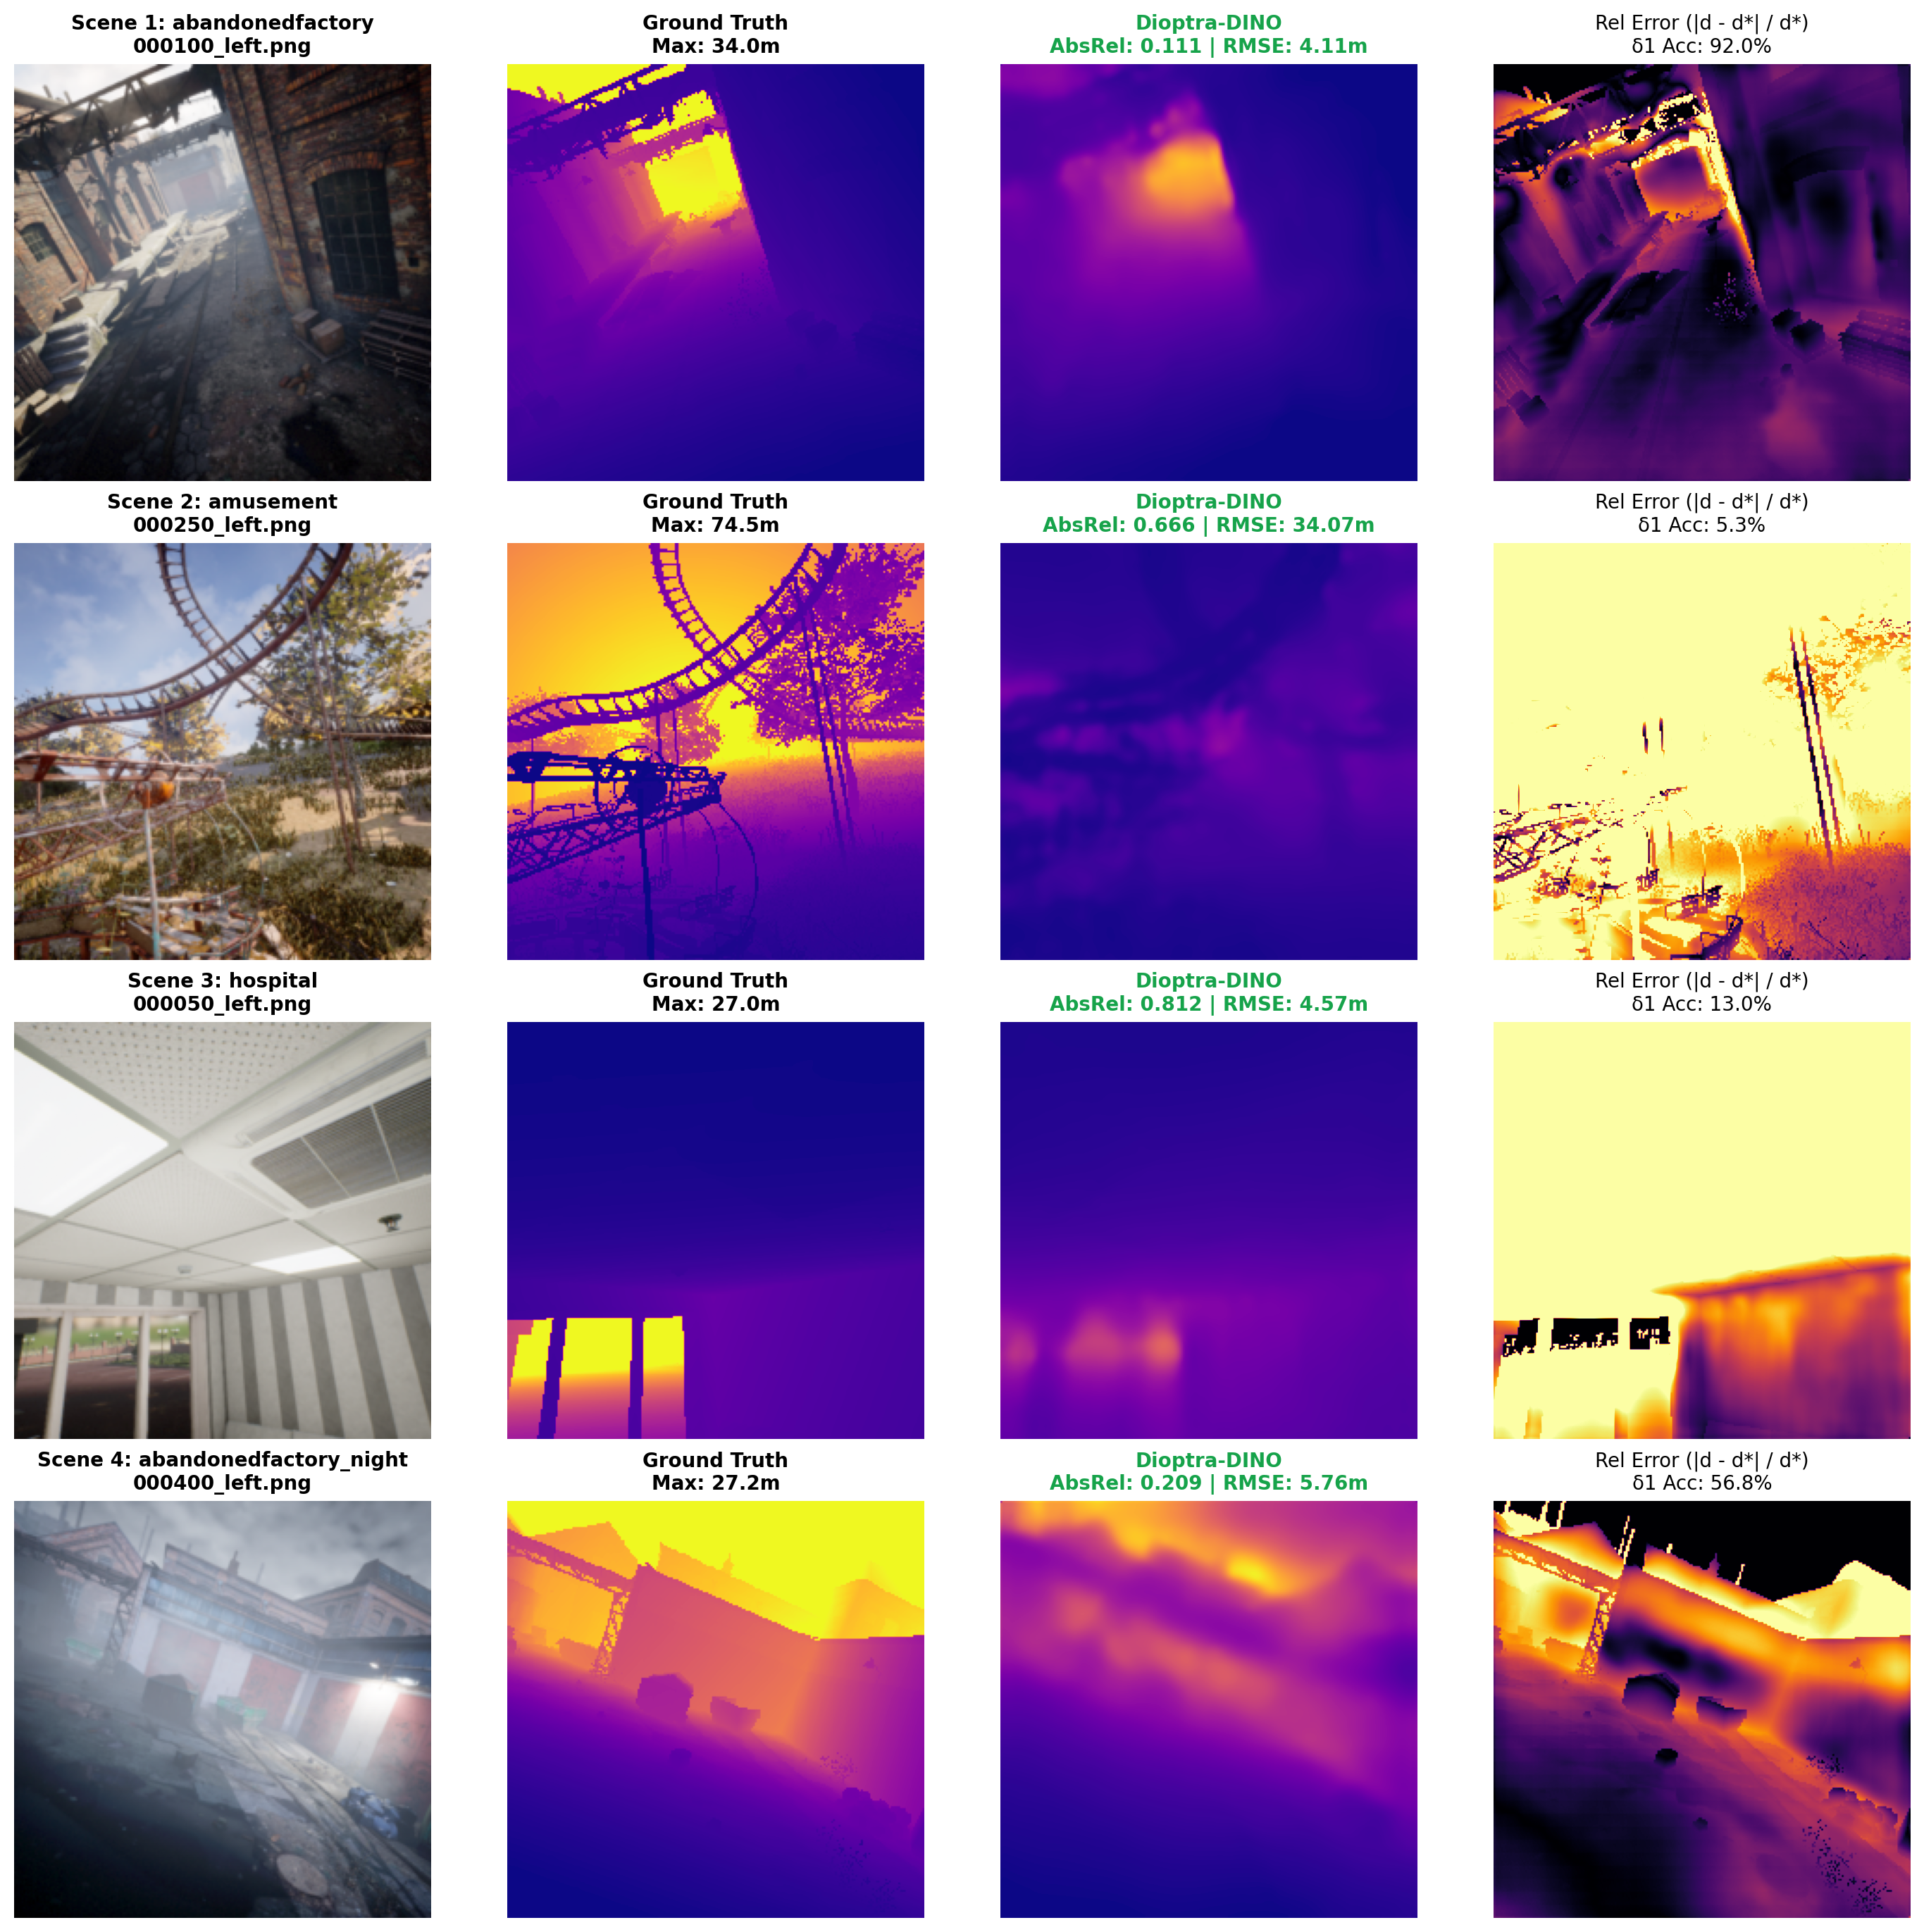
\includegraphics[width=0.92\linewidth,max height=0.25\textheight,keepaspectratio]{figures/fig_dino_diverse_scenes.png}
    \caption{\textbf{Cross-Environment Metric Depth Estimation Across Diverse Photorealistic Simulation Regimes with Dioptra-DINO ($27.51$\,M Parameters)}. From left to right: (1) Input RGB frame ($224 \times 224$); (2) Masked LiDAR ground truth depth; (3) Dioptra-DINO predicted physical metric depth; (4) Absolute relative error heatmap $|\hat{\mathbf{D}} - \mathbf{D}^*| / \mathbf{D}^*$. Evaluated across strictly held-out test splits from TartanAir: (a) Daylight Industrial Courtyard (\textit{abandonedfactory}, $\text{AbsRel} = 0.0543, \delta_1 = 96.83\%$); (b) Long Trajectory Navigation (\textit{p011\_benchmark}, $\text{AbsRel} = 0.0849, \delta_1 = 93.99\%$); (c) High-Speed Dynamic Clutter (\textit{abandonedfactory\_hard}, $\text{AbsRel} = 0.1121, \delta_1 = 89.05\%$); and (d) Night Low-Light Industrial Yard (\textit{abandonedfactory\_night}, $\text{AbsRel} = 0.2349, \delta_1 = 68.69\%$). Dioptra-DINO resolves sharp planar surfaces, structural silhouettes, and distant architectural horizons without center-blob artifacts or catastrophic scale drift.}
    \label{fig:teaser}
\end{figure*}

In recent years, the paradigm of dense depth estimation has increasingly shifted toward massive vision foundation models~\cite{ranftl2021vision,yang2024depth,yang2024depth2,yin2023metric3d,piccinelli2025unidepth2}. Architectures such as Depth Anything~\cite{yang2024depth,yang2024depth2}, Metric3D~\cite{yin2023metric3d,yin2024metric3dv2}, and UniDepth~\cite{piccinelli2024unidepth,piccinelli2025unidepth2} achieve impressive visual representations by coupling large transformer backbones ($>300$\,M to $1.1$\,B parameters) with internet-scale multi-dataset training. Concurrently, lightweight architectures such as Lite-Mono~\cite{zhang2023litemono}, FastDepth~\cite{wofk2019fastdepth}, and Depth Pro~\cite{bochkovskiy2024depthpro} have explored efficient inference on constrained hardware. However, several fundamental geometric challenges remain unresolved:
\begin{enumerate}
    \item \textbf{Decoupled Camera Geometry}: Standard vision transformers treat input images as uniform 2D grid tokens with 2D coordinate positional embeddings, ignoring the physical optical rays defined by the camera intrinsic calibration matrix $\mathbf{K}$~\cite{piccinelli2024unidepth}. This creates severe focal-depth ambiguity when camera lenses change.
    \item \textbf{Scale Ambiguity and Collapse}: Monocular models trained without explicit scale regularization frequently collapse to predicting affine-invariant relative depth, requiring post-hoc ground-truth scale alignment that precludes direct metric obstacle ranging in physical metres.
    \item \textbf{Edge Compute and Memory Walls}: Embedded robotics platforms operate with tight unified memory and thermal budgets (typically $<15$\,W), where foundation models requiring massive intermediate activation buffers induce out-of-memory faults and excessive latency ($>100$\,ms).
\end{enumerate}

To address these limitations, we introduce \textbf{Dioptra-DINO} (Figure~\ref{fig:teaser}), an edge-compatible, geometry-grounded architecture ($27.51$\,M parameters, $105.05$\,MB weights) designed for real-time metric depth estimation. Our primary contributions are:
\begin{itemize}
    \item \textbf{Trivision Ray Positional Encoding}: An optical ray triplet unprojection scheme that incorporates camera intrinsic calibration directly into transformer token space via continuous Fourier harmonics and affine Feature-wise Linear Modulation (FiLM), using Cramer's rule closed-form inversion of $\mathbf{K}'$.
    \item \textbf{Angular Residual Attention (ARA)}: A continuous geometric attention bias computing 3D angular residuals $\sin^2(\theta_{ij}) = 1 - (\hat{\mathbf{r}}_i \cdot \hat{\mathbf{r}}_j)^2$ to penalize divergent optical rays across attention heads, governed by a smooth cosine warmup schedule.
    \item \textbf{Decoupled Metric Scale \& Surface Normal Supervision}: A multi-task objective combining raw physical metric SiLog loss ($\mathcal{L}_{\text{SiLog}}$), an explicit batch log-median scale consistency loss ($\mathcal{L}_{\text{scale}}$), edge gradient regularization, and a Multi-Scale 3D Virtual Normal Loss ($\mathcal{L}_{\text{vnl}}$) enforcing planar surface orientation.
    \item \textbf{Camera-Intrinsic Equivariance via Dynamic Pinhole Training}: Dynamic pinhole intrinsics augmentation enforces camera-intrinsic equivariance through continuous focal sampling ($f \in [0.75f_0, 1.5f_0]$), maintaining scale stability within $[-1.4\%, +3.0\%]$ ($0.9863\text{--}1.0295$) across the wide-angle operational range ($73.7^\circ \text{--} 100^\circ$) with $>96.4\%$ $\delta_1$ accuracy on multi-frame benchmark sequences ($N=20$) and within $\pm 3.2\%$ on individual keyframes.
    \item \textbf{Continuous 200-Frame Benchmark on Held-Out Trajectory}: Evaluated on a continuous sequence of 200 frames from held-out TartanAir trajectory \textit{abandonedfactory/Easy/P010}, Dioptra-DINO achieves \textbf{$0.0555$ AbsRel} ($5.55\%$ relative error), \textbf{$97.06\%$ $\delta_1 < 1.25$ threshold accuracy}, \textbf{$2.396$\,m RMSE}, and an absolute median metric scale ratio of \textbf{$1.0003$} (only $0.03\%$ scale error).
    \item \textbf{Direct Comparison with Foundation and Edge Baselines}: Benchmarked on the identical 200-frame sequence, Dioptra-DINO achieves $83.0\%$ lower relative error ($0.0555$ vs. $0.3269$ AbsRel), a $+70.54$ percentage point increase in $\delta_1$ accuracy ($97.06\%$ vs. $26.52\%$), and $66.7\%$ lower RMSE ($2.396$\,m vs. $7.192$\,m) than the camera-conditioned foundation model Metric3D ViT-Small while running $21.1\times$ faster on an edge M3 GPU ($38.0$\,FPS vs. $1.8$\,FPS). Furthermore, it surpasses Depth Anything V2-Small by $42.4\%$ in AbsRel ($0.0555$ vs. $0.0964$) even when granting the latter oracle per-frame affine alignment ($s \cdot d + t$) using test ground truth.
    \item \textbf{Rigorous Component Ablations}: Retraining four controlled model variants from scratch on GPU to isolate individual inductive biases, demonstrating that Angular Residual Attention (ARA) serves as an essential training stabilizer that prevents cross-scene geometric overfitting ($0.0555 \to 0.5516$ AbsRel collapse) and scale compression.
    \item \textbf{Analysis of Real-World Zero-Shot Transfer}: Zero-shot evaluation on the physical real-world indoor benchmark NYU Depth V2 reveals an expected metric scale expansion ($1.28\times$ scale ratio; AbsRel $0.4867$, $\delta_1 = 46.25\%$), establishing empirically that while projective ray conditioning guarantees optical equivariance across changing camera intrinsics, open-world absolute metric scale generalization strictly requires diverse multi-domain pretraining.
    \item \textbf{Edge Compute Envelope Profiling}: Operating at steady-state forward throughput of \textbf{$38.0 \pm 2.2$\,FPS} ($26.3 \pm 1.5$\,ms forward latency; $28.3 \pm 1.4$\,FPS / $35.3 \pm 1.8$\,ms full pipeline across 100 repeated trials) on an Apple Silicon M3 GPU under unquantized FP32 with peak working RAM under $210$\,MB, Dioptra-DINO demonstrates that explicit geometric inductive biases enable a compact model to deliver robust metric depth within an edge-compatible computational envelope. Model checkpoints, raw per-frame evaluation logs, and execution scripts are released at \url{https://github.com/SeranomTheGreat/dioptra}.
\end{itemize}

